\section{Design}
\label{sec:design}

% --------------------------------------------------
\subsection{Contextual System}

To comply with the various shapes of knowledge context, there should be a feature system that can handle them.
It can be done with a major role of feature system that Satellid use called ``Contextual''.
The main ofsystem is by shortening the steps that needed to do a knowledge management that have context, with making it more effective and accessible.

\begin{figure}[htb]
    \centering
    % 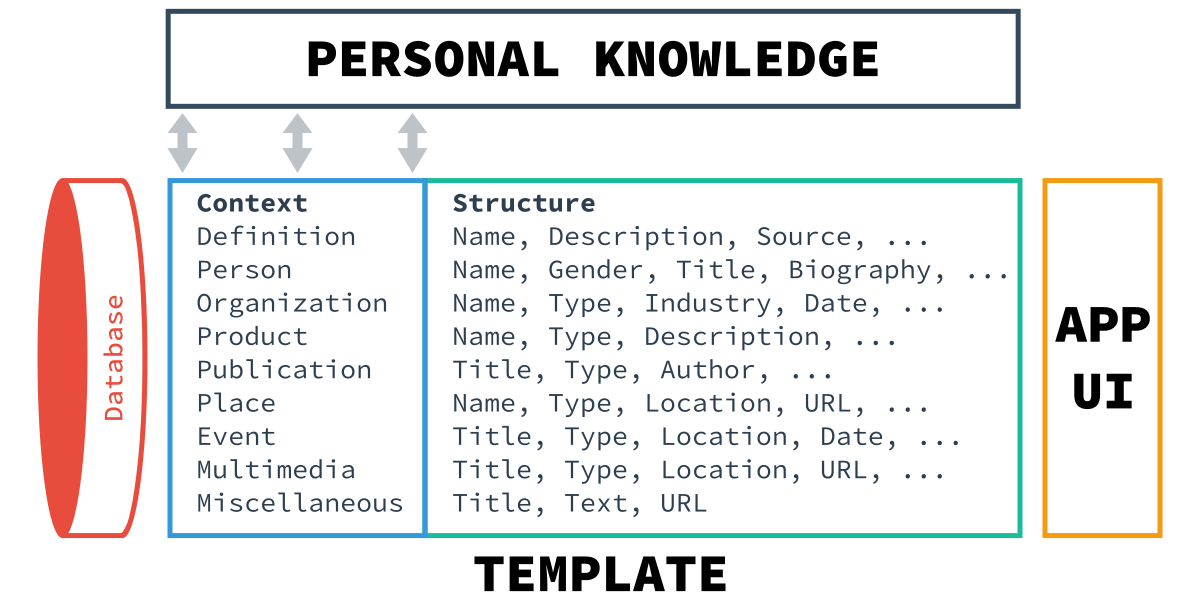
\includegraphics[width=\textwidth]{\dir/include/satellid-contextual}
    \caption{Contextual system visual representation}
    \label{fig:satellid-contextual}
\end{figure}

Contextual, illustrated as in \autoref{fig:satellid-contextual}, utilize inputted knowledge and template that are used together to form the context and structure.
With this, user will eventually always structure their data, and even create more or modify available data field.
In addition to this, category and tagging could also be built.
At the later time, it can be easily sorted faster than just using category or tags.
The difference of context with category or tag is how it handles specificity.
Context is very specific as a descriptor so it can be fully understood and assessed easily, rather than category or tag that is more widely and freely determined.
For example, \textit{The Merriam-Webster Dictionary} may be categorized as a ``dictionary'', ``book'', ``reference'', ``glossary'', ``thesaurus'' and tagged as ``word'', ``language'', ``english'', ``''; but its context basically just a ``publication''.
So it can be in the same context like \text{JavaScript, The Definitive Guide} or even \text{Iron Man comic}.
Contextual provide some of the most common type of knowledge with its key attributes.
The basic properties of metadata are including ID, Context, Date \& Time (Created \& Updated); while others are the Content or Detail.
As already defined, the lists below are the sorted version of prospected key attributes related to single context that needed and can be used.
Each of them can have category or label if appropriate, even additional custom text.
Also sometimes blank field is allowed like if there is unknown location and URL, while in other condition multiple entries could occur.

\begin{easylist}
& Definition
  && Name, Description, Source URL
& Person
  && Name (Full, First, Last, Nick), Gender, Birth Date or Age, Title (Job), Biography, Location (Address \& Coordinates), Phone, Email, Website, URL
& Organization
  && Name, Type (School, University, Institution, Company, Group, Community, Band), Industry, Date (Founded), Location (Address \& Coordinates), Product (their Services or Goods), URL
& Product
  && Name, Type (Service, Hardware, Software, Food, Clothing), Tagline, Description, Brand Detail, URL
& Publication
  && Title, Type (Article, Book, Paper, Dictionary, Novel, Tutorial, Comic, Website, Blog), Author, Description, URL
& Place
  && Name, Type (Station, Library, Park, Shop, Restaurant, Mall, Hotel, City, Country), Location (Address \& Coordinates), URL
& Event
  && Title, Type (Meetup, Seminar, Workshop, Conference, Festival), Location (Address), Date, Presenter, Sponsor, URL
& Multimedia
  && Title, Type (Photo, Image, Video, Film), Location, Date and Time (Published), Duration, Creator, URL
& Miscellaneous
  && Title, Text, URL
\end{easylist}

Other contexts that still classified as miscellaneous or mixed are like Story, Rules, Source Code, Prerequisites, Manifesto, etc.

% --------------------------------------------------
\subsection{Functionality Flow}

Since the primary reason to build the implementation of Satellid is to enable daily knowledge management for personal, the main focus to enable that person who frequently get knowledge or wanted to store their knowledge in a simple manner.
The primary functionality is to do \ac{BREAD}, also without having to bother the entries arrangement and everything is managed in a predefined context.
The application could be just deployable local network (easily also in their own computer) or accessed from the Web via Internet.
In a very simple way of interaction, it should be very intuitive.
To keep the process faster and shorter, all of the functional process can be done in one single interface layout of the application.
It all could happen with a simplified unified interface.
So there is no need to switch back and forth to different views of browse, search, read, edit, add, and delete.

\noindent There are some terminologies or parts of the interaction used in this flow, there are:

\begin{description}
\item [User]: The primary person who use Satellid
\item [System]: The Satellid application
\item [Database]: The databased that used by Satellid
\item [Knowledge]: The knowledge inside database that accessed and managed with Satellid
\item [Template]: The template to wrap the data schema
\item [Search bar]: The input that User can use to search for knowledge
\item [Buttons]: The input or modifier that User can use to add, edit, and delete a knowledge
\item [Knowledge]: The entity of knowledge, its object content
\item [Knowledge Collection]: The output that User can view the knowledge cards
\end{description}

\noindent The System will do the following flow:

\begin{enumerate}
\item System can be accessed and used by the User
\item System can run the desired interaction functionality by the User
\item System constantly monitor modification of Knowledge in the Database
\end{enumerate}

\noindent The User interactions are defined by these flow:

\begin{easylist}[enumerate]
& User can use, turn on and turn off the System
& User can interact with the System to:
  && Browse the stored Knowledge
  && Search a stored Knowledge
  && Read a stored Knowledge
  && Add a new Knowledge
  && Edit a stored Knowledge
  && Delete a stored Knowledge
& When User enter a text into the search bar:
  && Search a Knowledge based on typed text string
  && System search for matching text, automatically without having to press for a button
  && If matched Text is found, System show the search result
  && User get the found Knowledge
& When User click/tap the add button beside the search bar:
  && Add a new knowledge based on its context
  && User complete the new Knowldge
  && If new Knowledge is successfully inputted, System store the new Knowledge into the System
& When User click/tap the edit button beside the knowledge card:
  && Edit an existing knowledge
  && User edit the Knowldge
  && If the Knowledge is successfully edited, System store the edited Knowledge into the System
& When User click/tap the delete button beside the knowledge card:
  && Delete an existing knowledge
  && If the Knowledge is confirmed to be deleted, System delete the Knowledge from the System
\end{easylist}

% --------------------------------------------------
\subsection{Application Architecture}

As previously known, the application architecture is heavily based on Meteor platform.
It also covers its stack such as the JavaScript platform (Node.js), NoSQL database (MongoDB), reactive protocol (DDP).
All of them run in a regular web application environment, which there are client-side and server-side connected via a network that can be Internet or local network.
Based on simple web application architecture, the application is architected as in \autoref{fig:satellid-arch-app}.
% [?] inspired by

\begin{figure}[htbp]
    \centering
    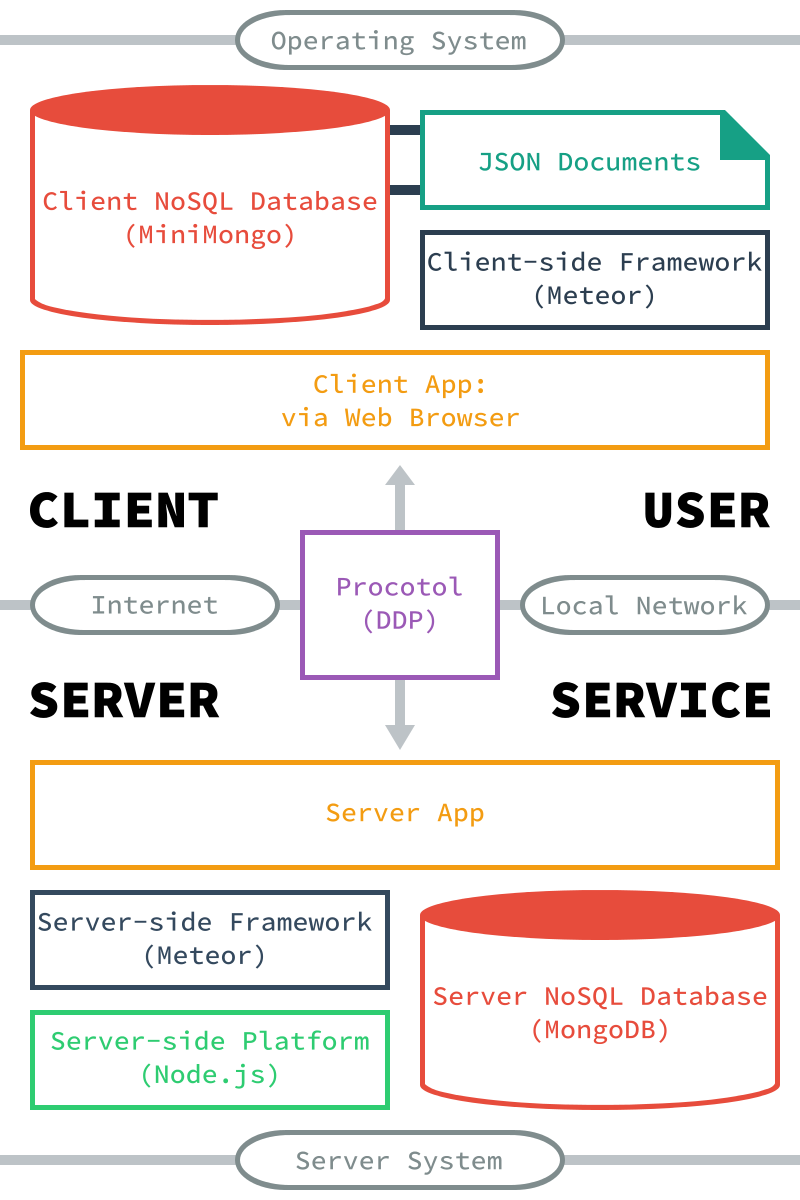
\includegraphics[width=8cm]{\dir/include/satellid-arch-app.png}
    \caption[Satellid Application Architecture]{The architecture of Satellid application}
    \label{fig:satellid-arch-app}
\end{figure}

The application started from the server system, running it including Node.js platform, Meteor platform, and server NoSQL database.
Those are served and accessed via the server-side app, naturally on top of a web server.
The application accessed by user from the client side, running it including Meteor app and client NoSQL database with \ac{JSON} documents that retrieved.
Those are accessible and enabled via client-side app, via the web browser.
Between the two, the protocol called \ac{DDP} maintain and manage the data transportation from server and client and from client to server.

% --------------------------------------------------
\subsection{User Interface and Interaction}

Here are the complete user interface and interaction on the web app version of Satellid.
The main interface or \ac{UI} design is laid out very simple, just like in \autoref{fig:satellid-ui}.

\begin{figure}[htb]
    \centering
    % \includegraphics[width=\textwidth]{\dir/include/satellid-ui}
    \caption{Main interface design of Satellid}
    \label{fig:satellid-ui}
\end{figure}

And then, the main interaction or \ac{UX} can be defined just like in \autoref{fig:satellid-ux}

%TODO User flow
\begin{figure}[htb]
    \centering
    % \includegraphics[width=\textwidth]{\dir/include/satellid-ux}
    \caption{Main interaction design of Satellid}
    \label{fig:satellid-ux}
\end{figure}
